% !TEX root = ../main.tex
\subsection{FMT Efficiency}
    % TODO. Explain 3 sources of low efficiency.

    % Low FMT efficiency + list sources.
    Compared to the alignment work described in section \ref{sec::fmtalignmentandreconstruction}, a low FMT is observed in this analysis.
    This can be seen in figure \ref{fig::vz_012933}.
    Upon inspection, three causes can be blamed for this: the application of incorrect alignment constants, a geometry effect, and a general FMT offline reconstruction issue.

    \begin{figure}[b!]
        \centering\frame{
        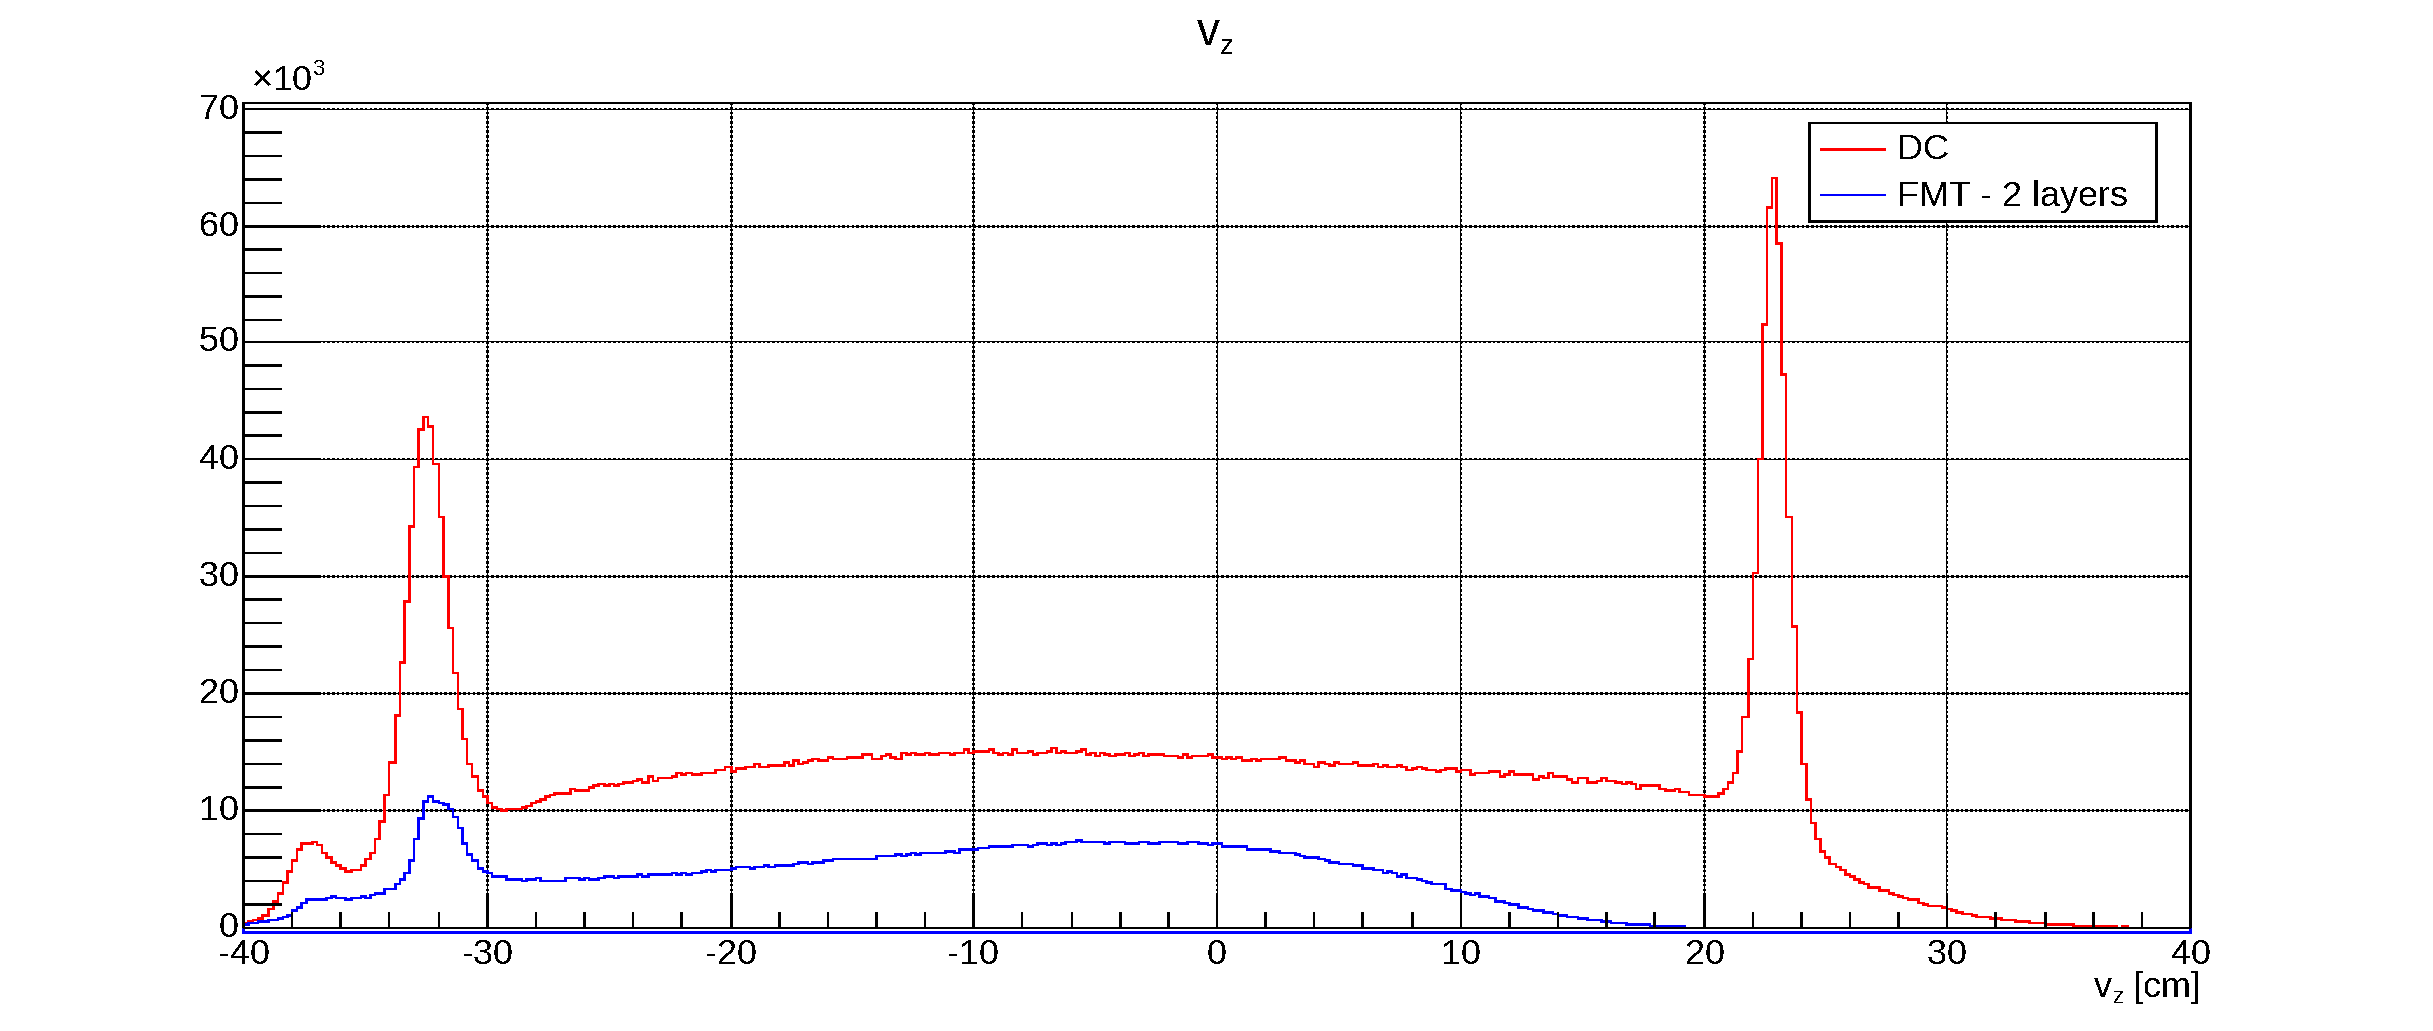
\includegraphics[width=\textwidth]{14resultsandconclusions/img/10vz_012933.pdf}}
        \caption[$v_z$ for DC and FMT, run 12933]{$v_z$ for DC (in red) and FMT (in blue). Summer 2020 data, run 12933. The wide peaks in FMT suggest an uncorrected misalignment.}
        \label{fig::vz_012933}
    \end{figure}

% --+ Alignment Effect +--------------------------------------------------------
    \subsubsection{Alignment Effect}
        % Introduction: The problem.
        The RG-F experiment's data is divided based on the season over which runs take place, thus there is Spring 2020 and Summer 2020 data.
        Based on the run group's guidelines, it is recommended to use Summer data, as it has seen more calibration than the Spring data.
        However, this calibration work hasn't included the FMT detector, and a strong misalignment effect is observed.

        % Cause of the problem.
        By simple visual inspection, two peaks can be clearly seen between $z = -36$ cm and $z = -30$ cm in figure \ref{fig::dc_vs_fmt_vz_011983}.
        These peaks are merged in figure \ref{fig::vz_012933}.
        As discussed in section \ref{sec::fmtalignmentandreconstruction}, this issue comes from a lack of correction for FMT misalignemnts.

        % Solution.
        The simplest solution is to use Spring data.
        While more work has been put on Summer data, it mainly pertains to the central detector; unrelated to this analysis.
        Figure \ref{fig::vz_012016} shows the same $v_z$ plot from Spring 2020 run 12016.
        Both peaks are clearly visible in this plot, suggesting that misalignments are properly accounted for in the run.

        \begin{figure}[t!]
            \centering\frame{
            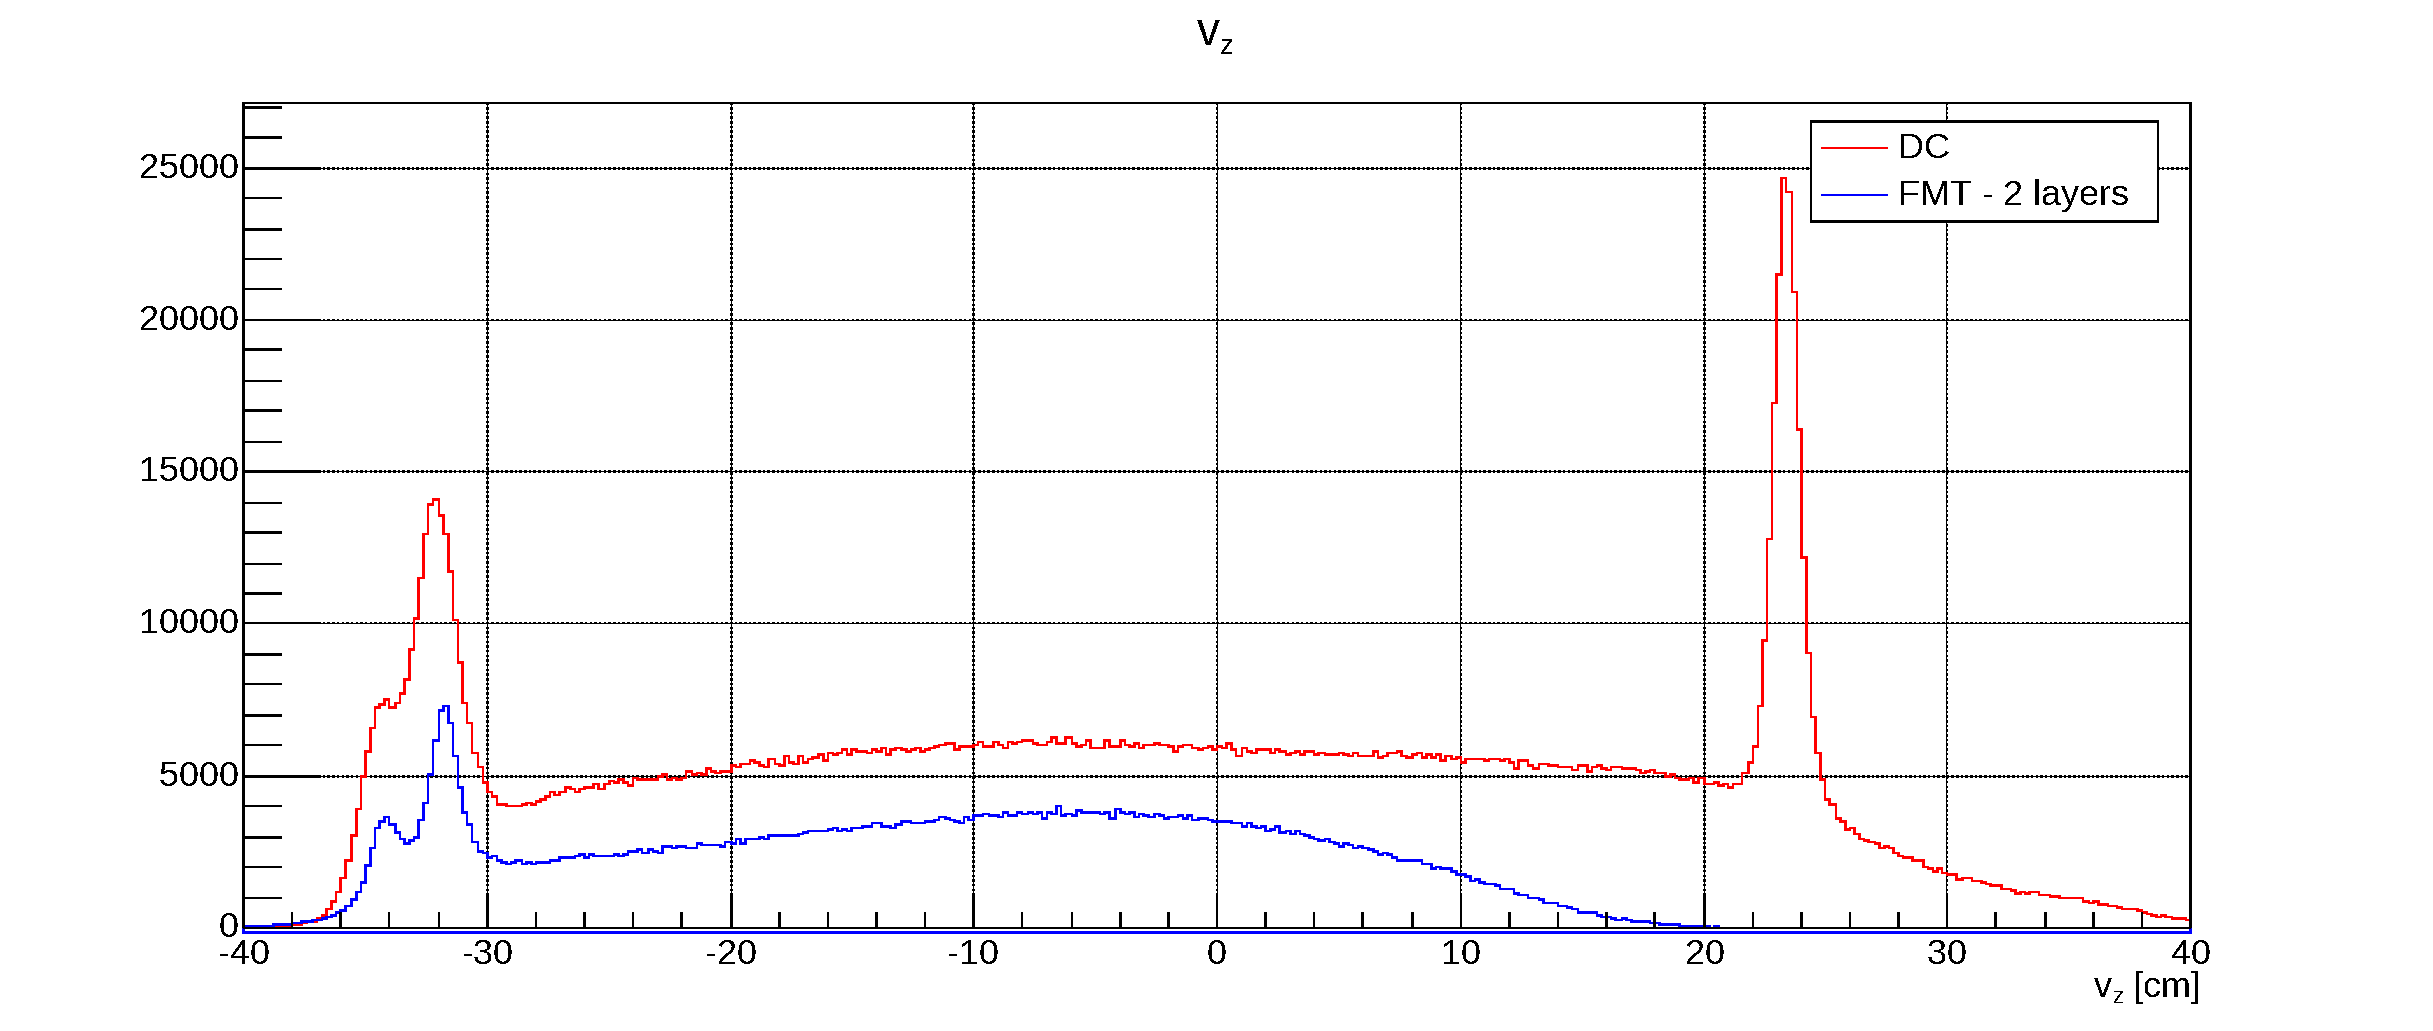
\includegraphics[width=\textwidth]{14resultsandconclusions/img/10vz_012016.pdf}}
            \caption[$v_z$ for DC and FMT, run 12016]{$v_z$ for DC (in red) and FMT (in blue). Spring 2020 data, run 12016. The upstream twin peaks can be clearly distinguished, suggesting a correct misalignment correction.}
            \label{fig::vz_012016}
        \end{figure}

% --+ Geometry Effect +---------------------------------------------------------
    \subsubsection{Geometry Effect}
        This problem is already discussed in detail in section \ref{ssec::validationandresults}.
        As a quick reminder, FMT sits at $z \approx 26$ cm, and it naturally performs poorly for targets to close to it.
        We can measure the strength of this effect by applying the geometry cut given by equation \eqref{eq::fmt_geometry_cut} to both DC and FMT tracks.
        Figure \ref{fig::vz_012016_geomcut} the effect of the cut when applied on figure \ref{fig::vz_012016}.
        Its effect on a $v_z$ vs $\theta$ plot can be seen on figure \ref{fig::vz_vs_theta}.

        \begin{figure}[h!]
            \centering\frame{
            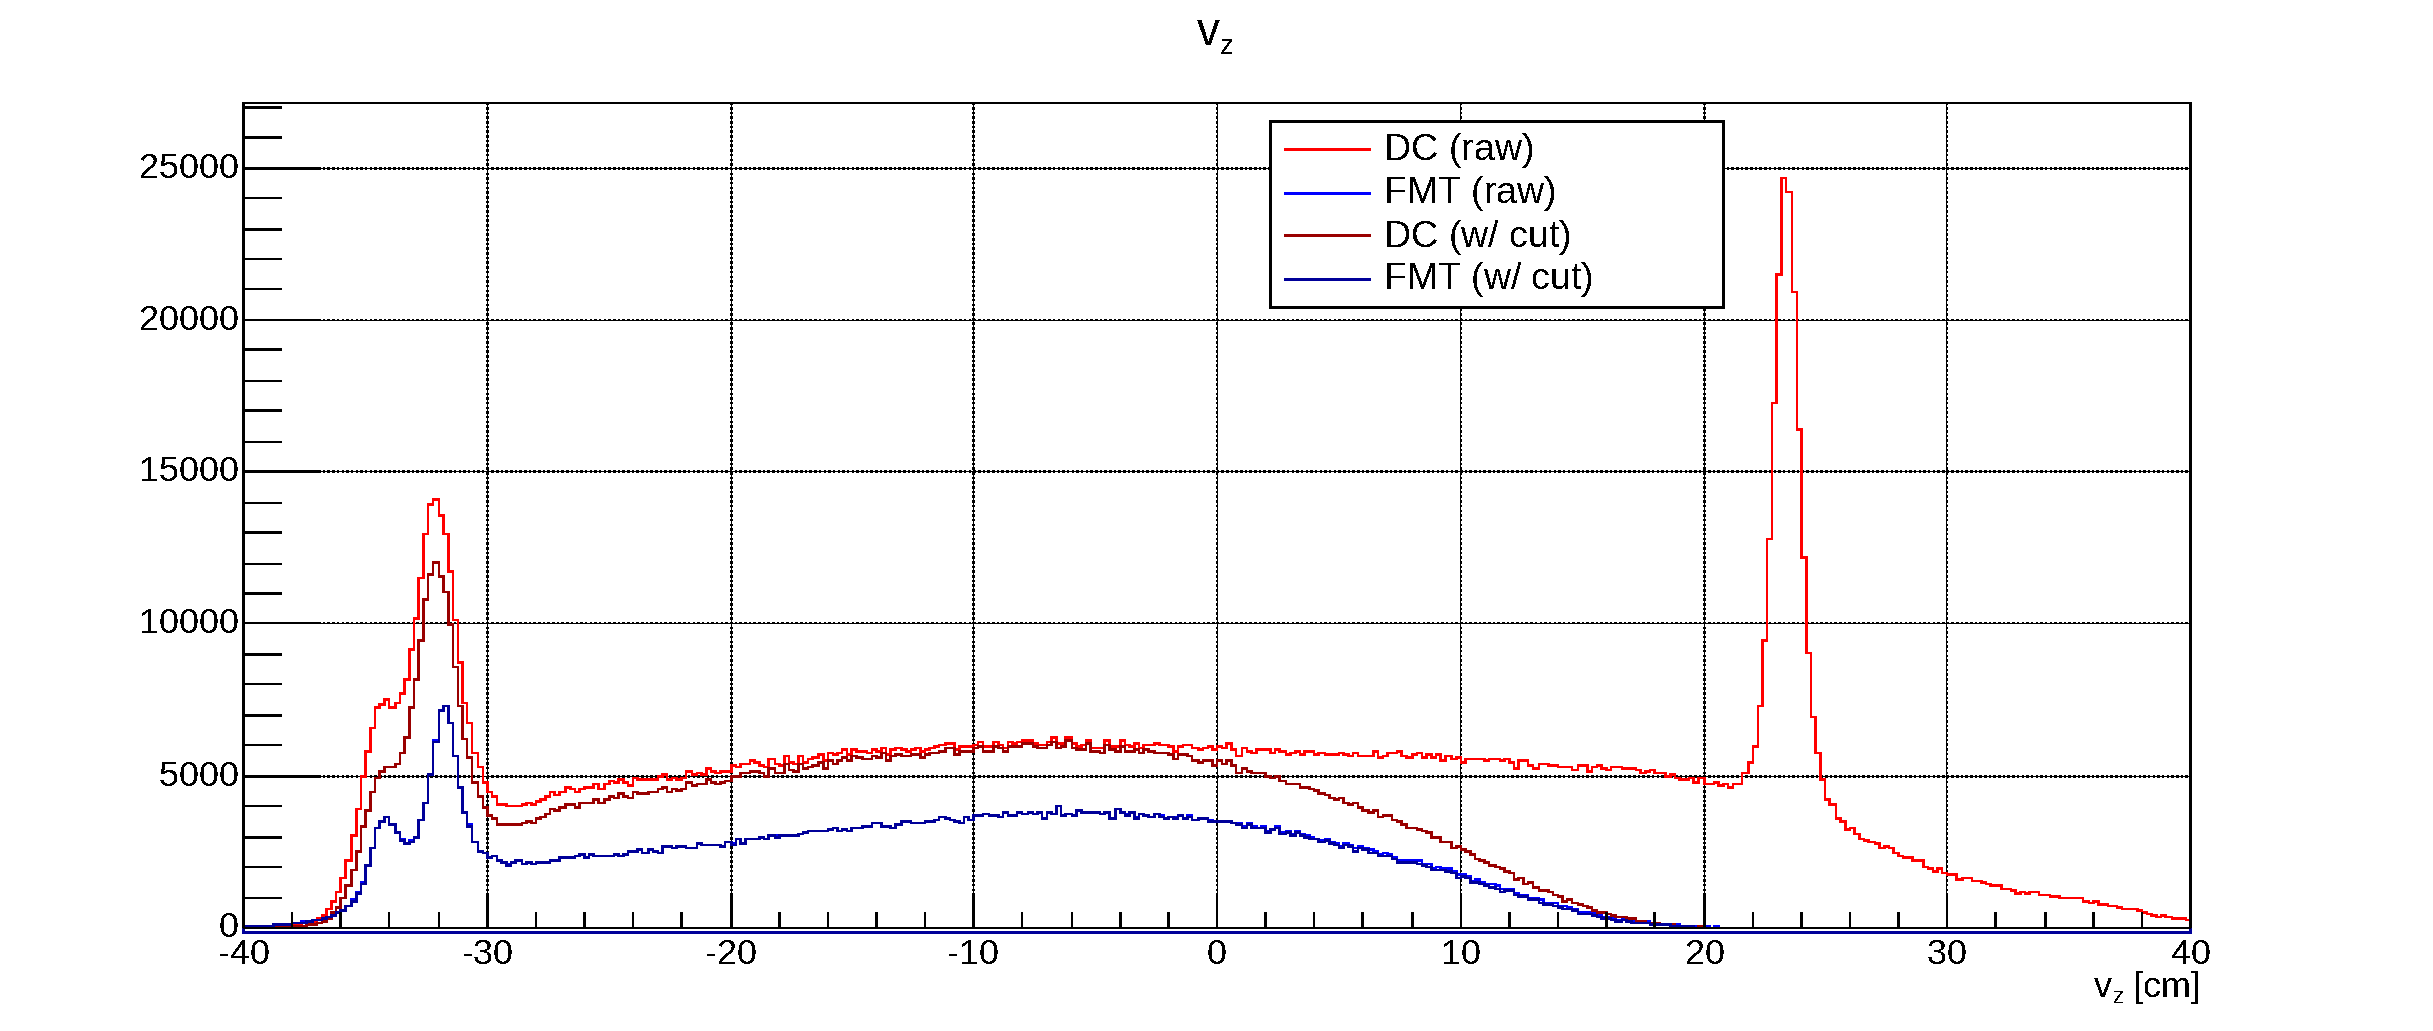
\includegraphics[width=\textwidth]{14resultsandconclusions/img/10vz_012016_geomcut.pdf}}
            \caption[$v_z$ for DC and FMT, w/ and w/out the geometry cut, run 12016]{$v_z$ for DC without the geometry cut (in red), with it (in dark red), for FMT without it (in blue), and with it (in dark blue). Spring 2020 data, run 12016. The effect is very clear on DC tracks, yet it almost doesn't affect FMT tracks.}
            \label{fig::vz_012016_geomcut}
        \end{figure}

% --+ Reconstruction Effect +---------------------------------------------------
    \subsubsection{Reconstruction Effect}
        % TODO.

% --+ Efficiency Study. +-------------------------------------------------------
    \subsubsection{Efficiency Study}
        % TODO. Add FMT efficiency study w/ and w/out geometry cut.
